\documentclass[11pt,twoside=semi,openright,numbers=noenddot,titlepage=false]{scrbook}
\newcommand{\napkinversion}{v0.1.\hbox{\the\year\twodigits\month\twodigits\day}}

%%fakesection Load packages

\usepackage{lmodern}
\usepackage[pdfusetitle]{hyperref}
\ExplSyntaxOn{}
\sys_if_engine_luatex:T {
	\usepackage{luatex85}
}
\sys_if_engine_pdftex:T {
	\usepackage[T1]{fontenc}
}
\ExplSyntaxOff{}

% These are evan.sty
\usepackage{amsmath,amssymb,amsthm}
\usepackage{mathrsfs}
\usepackage[svgnames,dvipsnames]{xcolor}
\usepackage{textcomp}
\usepackage{enumerate}
\usepackage[textsize=scriptsize,shadow]{todonotes}
\usepackage{mathtools}
\usepackage{microtype}
\usepackage[normalem]{ulem}
\usepackage{stmaryrd}
\usepackage{wasysym}
\usepackage{multirow}
\usepackage{prerex}
\usepackage[nameinlink]{cleveref}
\usepackage{derivative}
\usepackage{caption}
\usepackage{booktabs}
\usepackage{csquotes}

%%fakesection evan.sty macros
%Small commands
%% Napkin commands
\newcommand{\prototype}[1]{
	\emph{{\color{red} Prototypical example for this section:} #1} \par\medskip
}
\newenvironment{moral}{%
	\begin{tcolorbox}[boxrule=0.4pt,colframe=green!70!black,sharp corners,
		standard jigsaw,opacityback=0,left=10pt,right=10pt,top=3pt,bottom=3pt,
		before skip=10pt,after skip=20pt]%
	\bfseries\color{green!50!black}}%
	{\end{tcolorbox}}

%%fakesection Links (hyperref loaded earlier implicitly)
\hypersetup{
	linkcolor={red!50!black},
	citecolor={green!50!black},
	urlcolor={blue!80!black},
	pdfkeywords={napkin,math},
	pdfsubject={web.evanchen.cc},
	colorlinks,
}

%%fakesection Commutative diagrams
\usepackage{tikz-cd}
\usetikzlibrary{automata,positioning,arrows,arrows.meta,shapes}
\tikzset{
  ->, >=Stealth,
  node distance=2.5cm,
  every state/.style={thick, fill=blue!10},
  initial text={},
}
% make a larger hook
% https://tex.stackexchange.com/questions/514451/how-to-define-a-new-hooked-arrow
\makeatletter
\pgfdeclarearrow{
	name=xGlyph,
	cache=false,
	bending mode=none,
	parameters={\tikzcd@glyph@len,\tikzcd@glyph@shorten},
	setup code={%
		\pgfarrowssettipend{\tikzcd@glyph@len\advance\pgf@x{} by\tikzcd@glyph@shorten}},
	defaults={
		glyph axis=axis_height,
		glyph length=+1.55ex,
		glyph shorten=+-0.1ex},
	drawing code={%
		\pgfpathrectangle{\pgfpoint{+0pt}{+-1.5ex}}{\pgfpoint{+\tikzcd@glyph@len}{+3ex}}%
		\pgfusepathqclip%
		\pgftransformxshift{+\tikzcd@glyph@len}%
		\pgftransformyshift{+-\tikzcd@glyph@axis}%
		\pgftext[right,base]{\tikzcd@glyph}}}
\makeatother
\tikzcdset{
	arrow style=tikz,
	diagrams={>={Latex}},
	tikzcd left hook/.tip={xGlyph[glyph math command=supset, swap, glyph axis = 5.7pt]},
	tikzcd right hook/.tip={xGlyph[glyph math command=supset, glyph axis = 5.7pt]},
	surjective head arrow /.tip = {tikzcd to[sep=-1.5pt]tikzcd to},
	surjective head/.style={
		-surjective head arrow
	}
}

%%fakesection Page layout
\usepackage[headsepline]{scrlayer-scrpage}
\renewcommand{\headfont}{}
\addtolength{\textheight}{3.14cm}
\setlength{\footskip}{0.5in}
\setlength{\headsep}{10pt}

\def\shortdate{\leavevmode\hbox{\the\year-\twodigits\month-\twodigits\day}}
\def\twodigits#1{\ifnum#1<10 0\fi\the#1}
\automark[chapter]{chapter}

\rohead{\footnotesize\thepage}
\rehead{\footnotesize \textbf{\sffamily Napkin --- Computer Science Edition}, by \emph{Stevan Miladinovic} (\napkinversion)}
\lehead{\footnotesize\thepage}
\lohead{\footnotesize \leftmark}
\chead{}
\rofoot{}
\refoot{}
\lefoot{}
\lofoot{}
%\cfoot{\pagemark}

%%fakesection Fancy section and chapter heads
\renewcommand*{\sectionformat}{\color{purple}\S\thesection\autodot\enskip}
\renewcommand*{\subsectionformat}{\color{purple}\S\thesubsection\autodot\enskip}
\newcommand{\problemhead}{A few harder problems to think about}
\renewcommand{\thesubsection}{\thesection.\roman{subsection}}

\addtokomafont{chapterprefix}{\raggedleft}
\RedeclareSectionCommand[beforeskip=0.5em]{chapter}
\renewcommand*{\chapterformat}{%
\mbox{\scalebox{1.5}{\chapappifchapterprefix{\nobreakspace}}%
\scalebox{2.718}{\color{purple}\thechapter\autodot}\enskip}}

\addtokomafont{partprefix}{\rmfamily}
\renewcommand*{\partformat}{\color{purple}\scalebox{2.5}{\thepart}}

%%fakesection Theorems
\usepackage{tcolorbox}
\tcbuselibrary{breakable,skins,hooks}

% patch tcolorbox to support continuation of a paragraph
% after box
% from https://tex.stackexchange.com/questions/568782/
\makeatletter
\tcbset{
	after app={%
		\ifx\tcb@drawcolorbox\tcb@drawcolorbox@breakable{}
		\else
		% add only when not breakabel
		\@endparenv{}
		\fi
	}
}

% for breakable
\appto\tcb@use@after@lastbox{\@endparenv\@doendpe}
\makeatother
% END patch tcolorbox for continuation of paragraph


\usepackage{thmtools}

\theoremstyle{definition}
\declaretheoremstyle[
	headfont=\sffamily\bfseries\color{MidnightBlue},
	headpunct={\\[3pt]},
	postheadspace={0pt},
]{thmtheorem}


\declaretheoremstyle[
	headfont=\bfseries\color{RawSienna},
	headpunct={\\[3pt]},
	postheadspace={0pt},
]{thmexample}

\tcbset{
	theorem box/.style={
		enhanced,
		arc=9pt,
		outer arc=10pt,
		colframe=blue,
		colback=TealBlue!5,
		boxrule=1pt,
		before skip=12pt,
		after skip=14pt,
		left=10pt,
		right=10pt
	},
	remark box/.style={
		boxrule=0pt,
		frame hidden,
		sharp corners,
		enhanced,
		borderline west={2pt}{0pt}{ForestGreen},
		before skip=8pt,
		colback=ForestGreen!5,
		after skip=12pt,
		breakable,
		left=10pt,
		right=10pt
	},
	example box/.style={
		enhanced,
		sharp corners,
		arc=9pt,
		outer arc=10pt,
		colframe=RawSienna,
		colback=Salmon!5,
		boxrule=0.5pt,
		before skip=12pt,
		after skip=14pt,
		breakable,
		top=6pt,
		bottom=8pt,
		breakable,
		left=10pt,
		right=10pt
	},
	ques box/.style={
		boxrule=0pt,
		frame hidden,
		enhanced,
		sharp corners,
		before skip=8pt,
		after skip=12pt,
		borderline west={3pt}{0pt}{black},
		colback=RedViolet!5!gray!5,
		breakable,
		left=10pt,
		right=10pt
	}
}

\declaretheorem[style=thmtheorem,name=Theorem,numberwithin=section]{theorem}
\tcolorboxenvironment{theorem}{theorem box}
\declaretheorem[style=thmtheorem,name=Lemma,sibling=theorem]{lemma}
\tcolorboxenvironment{lemma}{theorem box}
\declaretheorem[style=thmtheorem,name=Proposition,sibling=theorem]{proposition}
\tcolorboxenvironment{proposition}{theorem box}
\declaretheorem[style=thmtheorem,name=Corollary,sibling=theorem]{corollary}
\tcolorboxenvironment{corollary}{theorem box}
\declaretheorem[style=thmexample,name=Example,sibling=theorem]{example}
\tcolorboxenvironment{example}{example box}

\declaretheoremstyle[
	headfont=\bfseries\sffamily\color{ForestGreen!70!black},
	bodyfont=\normalfont,
	headpunct={ --- },
]{thmremark}
\declaretheoremstyle[
	headfont=\bfseries\sffamily\color{ForestGreen!70!black},
	bodyfont=\normalfont,
	headpunct={},
]{thmremark*}

\declaretheoremstyle[
	headfont=\bfseries,
	bodyfont=\normalfont\small
]{thmques}

\declaretheorem[name=Question,sibling=theorem,style=thmques]{ques}
\tcolorboxenvironment{ques}{ques box}
\declaretheorem[name=Exercise,sibling=theorem,style=thmques]{exercise}
\tcolorboxenvironment{exercise}{ques box}
\declaretheorem[name=Remark,sibling=theorem,style=thmremark]{remark}
\tcolorboxenvironment{remark}{remark box}
\declaretheorem[name=Remark,sibling=theorem,style=thmremark*]{remark*}
\tcolorboxenvironment{remark*}{remark box}
\declaretheorem[name=Step,style=thmremark]{step} % only used in Lebesgue int
\tcolorboxenvironment{step}{remark box}

\theoremstyle{definition}
\newtheorem{claim}[theorem]{Claim}
\newtheorem{definition}[theorem]{Definition}
\newtheorem{fact}[theorem]{Fact}
\newtheorem{abuse}[theorem]{Abuse of Notation}

\newtheorem{problem}{Problem}[chapter]
\renewcommand{\theproblem}{\thechapter\Alph{problem}}
\newtheorem{sproblem}[problem]{Problem}
\newtheorem{dproblem}[problem]{Problem}
\renewcommand{\thesproblem}{\theproblem$^{\star}$}
\renewcommand{\thedproblem}{\theproblem$^{\dagger}$}
\newcommand{\listhack}{$\empty$\vspace{-2em}}

%%fakesection Answers
\usepackage{answers}
\Newassociation{hint}{answeritem}{tex/backmatter/all-hints}
\Newassociation{sol}{answeritem}{tex/backmatter/all-solns}
\renewcommand{\solutionextension}{out}
\renewenvironment{answeritem}[1]{\item[\bfseries #1.]}{}

%%fakesection Table of contents
% First add ToC to ToC
\makeatletter
\usepackage{etoolbox}
\pretocmd{\tableofcontents}{%
	\if@openright\cleardoublepage\else\clearpage\fi
	\pdfbookmark[0]{\contentsname}{toc}%
}{}{}%
\makeatother
\setcounter{tocdepth}{1}
\RedeclareSectionCommand[tocnumwidth=4.2em]{part}
\RedeclareSectionCommand[tocpagenumberwidth=2.2em,tocnumwidth=4.2em]{chapter}
\RedeclareSectionCommand[tocpagenumberwidth=2.2em,tocnumwidth=2.8em]{section}
% adjust tocpagenumberwidth manually for large page number: https://tex.stackexchange.com/a/502168

%%fakesection Asymptote definitions
\usepackage{patch-asy}
\numberwithin{asy}{chapter}
\renewcommand{\theasy}{\thechapter\Alph{asy}}
\begin{asydef}
	import extras;
	size (6cm);
	usepackage ('amsmath');
	usepackage ('amssymb');
	defaultpen (fontsize (11pt));
	settings.tex = `latex';
	settings.outformat = `pdf';
\end{asydef}
\def\asydir{asy}

%%fakesection Bibliography
\usepackage[backend=biber,backref=true,style=alphabetic]{biblatex}
\DeclareLabelalphaTemplate{
	\labelelement{
		\field[final]{shorthand}
		\field{label}
		\field[strwidth=2,strside=left]{labelname}
	}
	\labelelement{
		\field[strwidth=2,strside=right]{year}
	}
}
\DeclareFieldFormat{labelalpha}{\textbf{\scriptsize #1}}
\addbibresource{references.bib}
\addbibresource{images.bib}
%% stylistic biblatex choices
\DefineBibliographyStrings{english}{%
	backrefpage  = {cited p.}, % for single page number
	backrefpages = {cited pp.} % for multiple page numbers
}
\DeclareFieldFormat{journaltitle}{\mkbibemph{#1},} % italic journal title with comma
\DeclareFieldFormat[inbook,thesis]{title}{\mkbibemph{#1}\addperiod} % italic title with period
\DeclareFieldFormat[article]{title}{#1} % title of journal article is printed as normal text
\DeclareFieldFormat[article]{volume}{\textbf{#1}\addcolon\space}
\renewcommand{\mkbibnamegiven}[1]{\textsc{#1}}
\renewcommand{\mkbibnamefamily}[1]{\textsc{#1}}
\renewcommand{\mkbibnameprefix}[1]{\textsc{#1}}
\renewcommand{\mkbibnamesuffix}[1]{\textsc{#1}}
\renewcommand{\finentrypunct}{}

%%fakesection Mini ToC
\usepackage[tight]{minitoc}
\mtcsetfont{parttoc}{chapter}{\sffamily\bfseries}
\mtcsetfont{parttoc}{section}{\footnotesize\rmfamily\upshape\mdseries}
\mtcsetfont{parttoc}{subsection}{\footnotesize\rmfamily\upshape\mdseries}
%\mtcsetdepth{parttoc}{1}
\setcounter{parttocdepth}{1}
\renewcommand*{\partheadstartvskip}{\vspace*{20em}}
\renewcommand*{\partheadendvskip}{}
%\noptcrule
\renewcommand\beforeparttoc{\noindent{\bfseries \Large Part \thepart: Contents}}
%\hspace{\fill}\rule{0.95\linewidth}{2pt}\hspace{\fill}
\doparttoc[n]

%%fakesection Misc haxx
\pdfstringdefDisableCommands{\def\Spec{\text{Spec }}\def\sigma{σ}}

\DeclareBibliographyDriver{image}{%
  \usebibmacro{author/editor}%
  \newunit\newblock{}
  \printfield{title}%
  \newunit\newblock{}
  \printfield{year}%
  \newunit\newblock{}
  \printfield{url}%
  \newunit\newblock{}
  \iffieldundef{urldate}
    {}
    {\mkbibparens{Accessed: \printfield{urldate}}}%
  \finentry{}
}

\newcommand{\cbrt}[1]{\sqrt[3]{#1}}
\newcommand{\floor}[1]{\left\lfloor{} #1 \right\rfloor}
\newcommand{\ceiling}[1]{\left\lceil{} #1 \right\rceil}
\newcommand{\mailto}[1]{\href{mailto:#1}{\texttt{#1}}}
\newcommand{\ol}{\overline}
\newcommand{\ul}{\underline}
\newcommand{\wt}{\widetilde}
\newcommand{\wh}{\widehat}
\newcommand{\eps}{\varepsilon}
%\renewcommand{\iff}{\Leftrightarrow}
%\renewcommand{\implies}{\Rightarrow}
\newcommand{\vocab}[1]{\textbf{\color{blue} #1}}
\newcommand{\catname}{\mathsf}
\newcommand{\hrulebar}{
  \par\hspace{\fill}\rule{0.95\linewidth}{.7pt}\hspace{\fill}
  \par\nointerlineskip{}\vspace{\baselineskip}
}
\newcommand{\half}{\frac{1}{2}}

%More commands and math operators
\DeclareMathOperator{\cis}{cis}
\DeclareMathOperator*{\lcm}{lcm}
\DeclareMathOperator*{\argmin}{arg min}
\DeclareMathOperator*{\argmax}{arg max}

%Convenient Environments
\newenvironment{soln}{\begin{proof}[Solution]}{\end{proof}}
\newenvironment{parlist}{\begin{inparaenum}[(i)]}{\end{inparaenum}}
\newenvironment{gobble}{\setbox\z@\vbox\bgroup}{\egroup}

%Inequalities
\newcommand{\cycsum}{\sum_{\mathrm{cyc}}}
\newcommand{\symsum}{\sum_{\mathrm{sym}}}
\newcommand{\cycprod}{\prod_{\mathrm{cyc}}}
\newcommand{\symprod}{\prod_{\mathrm{sym}}}

%From H113 "Introduction to Abstract Algebra" at UC Berkeley
\newcommand{\CC}{\mathbb{C}}
\newcommand{\FF}{\mathbb{F}}
\newcommand{\NN}{\mathbb{N}}
\newcommand{\QQ}{\mathbb{Q}}
\newcommand{\RR}{\mathbb{R}}
\newcommand{\ZZ}{\mathbb{Z}}
\newcommand{\charin}{\text{ char }}
\DeclareMathOperator{\sign}{sign}
\DeclareMathOperator{\Aut}{Aut}
\DeclareMathOperator{\Inn}{Inn}
\DeclareMathOperator{\Syl}{Syl}
\DeclareMathOperator{\Gal}{Gal}
\DeclareMathOperator{\GL}{GL} % General linear group
\DeclareMathOperator{\SL}{SL} % Special linear group

%From Kiran Kedlaya's "Geometry Unbound"
\newcommand{\abs}[1]{\left\lvert{} #1 \right\rvert}
\newcommand{\norm}[1]{\left\lVert{} #1 \right\rVert}
\newcommand{\dang}{\measuredangle} %% Directed angle
\newcommand{\ray}[1]{\overrightarrow{#1}}
\newcommand{\seg}[1]{\overline{#1}}
\newcommand{\arc}[1]{\wideparen{#1}}

%From M275 "Topology" at SJSU
\newcommand{\id}{\mathrm{id}}
\newcommand{\taking}[1]{\xrightarrow{#1}}
\newcommand{\inv}{^{-1}}

%From M170 "Introduction to Graph Theory" at SJSU
\DeclareMathOperator{\diam}{diam}
\DeclareMathOperator{\ord}{ord}
%\newcommand{\defeq}{\overset{\mathrm{def}}{=}}
\newcommand{\defeq}{\coloneq}

%From the USAMO .tex files
\newcommand{\st}{^{\text{st}}}
\newcommand{\nd}{^{\text{nd}}}
\renewcommand{\th}{^{\text{th}}}
\newcommand{\dg}{^\circ}
\newcommand{\ii}{\item}

% From Math 55 and Math 145 at Harvard
\newenvironment{subproof}[1][Proof]{%
\begin{proof}[#1] \renewcommand{\qedsymbol}{$\blacksquare$}}%
{\end{proof}}

\newcommand{\liff}{\leftrightarrow}
\newcommand{\lthen}{\rightarrow}
\newcommand{\opname}{\operatorname}
\newcommand{\surjto}{\twoheadrightarrow}
\newcommand{\injto}{\hookrightarrow}
\newcommand{\On}{\mathrm{On}} % ordinals
\DeclareMathOperator{\img}{im} % Image
\DeclareMathOperator{\Img}{Im} % Image
\DeclareMathOperator{\coker}{coker} % Cokernel
\DeclareMathOperator{\Coker}{Coker} % Cokernel
\DeclareMathOperator{\Ker}{Ker} % Kernel
\DeclareMathOperator{\rank}{rank}
\DeclareMathOperator{\Spec}{Spec} % spectrum
\DeclareMathOperator{\Tr}{Tr} % trace
\DeclareMathOperator{\pr}{pr} % projection
\DeclareMathOperator{\ext}{ext} % extension
\DeclareMathOperator{\pred}{pred} % predecessor
\DeclareMathOperator{\dom}{dom} % domain
\DeclareMathOperator{\ran}{ran} % range
\DeclareMathOperator{\Hom}{Hom} % homomorphism
\DeclareMathOperator{\End}{End} % endomorphism

% Things Lie
\newcommand{\kg}{\mathfrak{g}}
\newcommand{\kh}{\mathfrak{h}}
\newcommand{\kn}{\mathfrak{n}}
\newcommand{\ku}{\mathfrak{u}}
\newcommand{\kz}{\mathfrak{z}}
\DeclareMathOperator{\Ext}{Ext} % Ext functor
\DeclareMathOperator{\Tor}{Tor} % Tor functor

% More script letters etc.
\newcommand{\SA}{\mathscr{A}}
\newcommand{\SB}{\mathscr{B}}
\newcommand{\SC}{\mathscr{C}}
\newcommand{\SD}{\mathscr{D}}
\newcommand{\SF}{\mathscr{F}}
\newcommand{\SG}{\mathscr{G}}
\newcommand{\SH}{\mathscr{H}}
\newcommand{\OO}{\mathcal{O}}


%%fakesection Napkin Macros
\newcommand{\Zc}[1]{\ZZ/#1\ZZ}
\newcommand{\Zcc}[1]{\ZZ/ (#1) \ZZ}
\newcommand{\Zm}[1]{(\ZZ/#1\ZZ)^\times}
\newcommand{\EE}{\mathbb{E}}
\newcommand{\TT}{\mathbb{T}}
\newcommand{\im}{^{\text{img}}} % or ``?
\newcommand{\pre}{^{\text{pre}}}
\newcommand{\normalin}{\trianglelefteq}
\newcommand{\triv}{\mathrm{triv}}
\newcommand{\largeotimes}[1]{\mathop{\otimes}\limits_{#1}}
\newcommand{\Mat}{\mathrm{Mat}}
\newcommand{\PGL}[1]{\mathbf{PGL}_{#1} (\CC)}

\DeclareMathOperator{\Stab}{Stab}
\DeclareMathOperator{\FixPt}{FixPt}
\DeclareMathOperator{\refl}{refl}
\DeclareMathOperator{\Fun}{Fun}
\DeclareMathOperator{\Irrep}{Irrep}
\DeclareMathOperator{\Res}{Res}
\DeclareMathOperator{\Reg}{Reg}
\DeclareMathOperator{\Classes}{Classes}
\DeclareMathOperator{\Frac}{Frac}
\newcommand{\FunCl}{\Fun_{\mathrm{class}}}
\newcommand{\Homrep}{\Hom_{\mathrm{rep}}}
\newcommand{\ab}{^\text{ab}} % abelianization
\DeclareMathOperator{\ev}{ev}
\DeclareMathOperator{\Wind}{\mathbf{I}}
\newcommand{\Ctriv}{\CC_{\mathrm{triv}}}
\newcommand{\Csign}{\CC_{\mathrm{sign}}}
\DeclareMathOperator{\Alt}{Alt}

% Riemann surface
\DeclareMathOperator{\Div}{div} % divisor
\DeclareMathOperator{\mult}{mult}

% Alg geom macros
\newcommand{\VV}{\mathcal{V}}
\newcommand{\Vp}{\mathcal{V}_{\text{pr}}}
\newcommand{\Aff}{\mathbb{A}}
\newcommand{\II}{\mathcal{I}_{\text{rad}}}
\newcommand{\RP}{\mathbb{RP}}
\newcommand{\CP}{\mathbb{CP}}
\newcommand{\Cl}{\mathrm{Cl}}
\newcommand{\restrict}[1]{\bgroup\restriction_{#1}\egroup}
\DeclareMathOperator{\Opens}{OpenSets}
\DeclareMathOperator{\Proj}{Proj}
\DeclareMathOperator{\res}{res}
\newcommand{\km}{\mathfrak{m}}
\newcommand{\sh}{^\mathrm{sh}}

\renewcommand{\Re}{\opname{Re}}
\renewcommand{\Im}{\opname{Im}}

%% Category Theory macros
\renewcommand{\AA}{\mathcal{A}}
\newcommand{\BB}{\mathcal{B}}
\newcommand{\obj}{\operatorname{obj}}
\newcommand{\op}{^{\mathrm{op}}}


\usepackage{tkz-graph}
\pgfarrowsdeclare{biggertip}{biggertip}{%
  \setlength{\arrowsize}{1pt}
  \addtolength{\arrowsize}{.1\pgflinewidth}
  \pgfarrowsrightextend{0}
  \pgfarrowsleftextend{-5\arrowsize}
}{%
  \setlength{\arrowsize}{1pt}
  \addtolength{\arrowsize}{.1\pgflinewidth}
  \pgfpathmoveto{\pgfpoint{-5\arrowsize}{4\arrowsize}}
  \pgfpathlineto{\pgfpointorigin}
  \pgfpathlineto{\pgfpoint{-5\arrowsize}{-4\arrowsize}}
  \pgfusepathqstroke{}
}
\tikzset{
	EdgeStyle/.style = {>=biggertip}
}

\usepackage[all,cmtip,2cell]{xy}
\UseTwocells{}
\newcommand\nattfm[5]{\xymatrix@C+2pc{#1 \rtwocell<4>^{#2}_{#4}{\; #3} & #5}}

%% Alg Top macros
\DeclareMathOperator{\Cells}{Cells}
\newcommand{\HdR}{H_{\mathrm{dR}}}

%% Alg NT macros
\newcommand{\ka}{\mathfrak{a}}
\newcommand{\kb}{\mathfrak{b}}
\newcommand{\kp}{\mathfrak{p}}
\newcommand{\kq}{\mathfrak{q}}

\newcommand{\Frob}{\mathrm{Frob}}
\DeclareMathOperator{\Norm}{N}
\DeclareMathOperator{\Ram}{Ram}
\newcommand{\TrK}{\Tr_{K/\QQ}}
\newcommand{\NK}{\Norm_{K/\QQ}}
\newcommand{\kf}{\mathfrak{f}}
\newcommand{\kP}{\mathfrak{P}}
\newcommand{\kQ}{\mathfrak{Q}}

%% Diff geo macros
\newcommand{\ee}{\mathbf{e}}
\newcommand{\fpartial}[2]{\frac{\partial{}#1}{\partial{}#2}}

%% ST macros
\newcommand{\CH}{\mathsf{CH}}
\newcommand{\ZFC}{\mathsf{ZFC}}

\newcommand{\Name}{\text{Name}}
\newcommand{\Po}{\mathbb{P}}
\newcommand{\nrank}{\opname{n-rank}} % ranks
\newcommand{\PP}{\mathcal{P}}

\newcommand{\EmptySet}{\mathrm{EmptySet}}
\newcommand{\PowerSet}{\mathrm{PowerSet}}
\newcommand{\Pairing}{\mathrm{Pairing}}
\newcommand{\Infinity}{\mathrm{Infinity}}
\newcommand{\Extensionality}{\mathrm{Extensionality}}
\newcommand{\Foundation}{\mathrm{Foundation}}
\newcommand{\Union}{\mathrm{Union}}
\newcommand{\Comprehension}{\mathrm{Comprehension}}
\newcommand{\Replacement}{\mathrm{Replacement}}

%% New macros
\newcommand{\symdif}{\Delta}
\newcommand{\xor}{\oplus}

\usepackage{mathrsfs}

\newcommand\MM{\mathscr{M}}
\newcommand\llex{<_{\text{lex}}}

\DeclareMathOperator{\cof}{cof}

%% Quantum macros
\usepackage{braket}
\newcommand{\cvec}[1]{\begin{bmatrix} #1 \end{bmatrix}}
\newcommand{\pair}[2]{\begin{bmatrix} #1 \\ #2 \end{bmatrix}}
\newcommand{\zup}{\ket\uparrow}
\newcommand{\zdown}{\ket\downarrow}
\newcommand{\xup}{\ket\rightarrow}
\newcommand{\xdown}{\ket\leftarrow}
\newcommand{\yup}{\ket\otimes}
\newcommand{\ydown}{\ket\odot}
\newcommand{\UCNOT}{U_{\mathrm{CNOT}}}
\newcommand{\UQFT}{U_{\mathrm{QFT}}}

%% Measure
\DeclareMathOperator{\Var}{Var}
\newcommand{\cme}{^\text{cm}}
\newcommand{\asto}{\xrightarrow{\text{a.s.}}}

%% Hot chili peppers
\reversemarginpar{}
\newcommand{\prechili}{\vspace*{0.3em}\hspace*{\fill}}
\newcommand{\chili}{
\includegraphics[width=1.5em]{media/chili.png}}
\newcommand{\onechili}{\marginpar{\prechili\chili}}
\newcommand{\twochili}{\marginpar{\prechili\chili\chili}}
\newcommand{\threechili}{\marginpar{\prechili\chili\chili\chili}}

%% Relations
\newcommand{\ovalrelation}[5]{%
  \begin{scope}[xshift=#1, yshift=#2]
    % Draw ovals
    \node[draw, color=black!0, fill=blue!20, ellipse, minimum width=1.6cm, minimum height=4cm] (D) at (0,0) {};
    \node[draw, color=black!0, fill=red!20, ellipse, minimum width=1.6cm, minimum height=4cm] (C) at (4,0) {};

    % Domain points
    \foreach \y [count=\i] in {#3} {
      \node[circle, fill=gray!50, inner sep=2pt] (d\i) at (0,\y) {};
    }

    % Codomain points
    \foreach \y [count=\i] in {#4} {
      \node[circle, fill=gray!50, inner sep=2pt] (c\i) at (4,\y) {};
    }

    % Arrows and coloring
    \foreach \d/\c in {#5} {
      \draw[-{Latex[width=1.2mm]}, thick] (d\d) -- (c\c);
      \node at (d\d) [circle, fill=blue!70, inner sep=2pt] {};
      \node at (c\c) [circle, fill=red!70, inner sep=2pt] {};
    }
  \end{scope}
}


\title{An Infinitely Large Napkin}
\subtitle{Computer Science Edition}
\author{Stevan Miladinovic}
\date{Version: \napkinversion}

\begin{document}

\frontmatter
% \renewcommand{\thepage}{\arabic{page}}
\maketitle

\bgroup{}
\fboxrule=4pt
%\noindent\fbox{\includegraphics[width=\textwidth]{cover-art.jpg}}
\egroup{}
\newpage

\begin{titlepage}
	\vspace*{3cm}
	\begin{flushright}
		\large\itshape
		When introduced to a new idea, always ask why you should care. \\[0.2cm]
		Do not expect an answer right away, but demand one eventually. \\[0.8cm]
		--- Ravi Vakil~\cite{ref:vakil}
	\end{flushright}

	\vfill
	{
	\small
    \noindent \emph{This Book is inspired by Evan Chen's ``An Infinitely Large
      Napkin''\cite{ref:napkin}.} \\[0.4cm]
	\noindent {\copyright} \the\year{} Stevan Miladinovic. \\
	Text licensed under
	\href{https://creativecommons.org/licenses/by-sa/4.0/}{CC-by-SA-4.0}.
	Source files licensed under
	\href{https://choosealicense.com/licenses/gpl-3.0/}{GNU GPL v3}.
	\\[0.4cm]
	This is (still!)\ an \textbf{incomplete draft}.
	Please send corrections, comments,
	etc.\ to \mailto{cs.napkin@gmail.com},
	or pull-request at \url{https://github.com/StevanMiladinovic/napkin-cs}.
	\\[0.4cm]
	\noindent Last updated \today.
	\vspace*{1cm}
	}
\end{titlepage}

% TODO: \include{tex/frontmatter/preface}

\setcounter{chapter}{-1} % avoid sales pitch collision
%\addtocounter{chapter}{-1}
\chapter{Advice for the Reader}

\section{Prerequisites}
This book is intended to be accessible to anyone with a basic understanding of
high school level mathematics.
In particular, the reader is not expected to know anything about higher maths,
computer science or programming.

Some fundamental ideas that surpass this scope shall be introduced in
\Cref{part:foundations}. If you already understand them,
you are welcome to skip this part.

\section{Deciding What to Read}
There is no need to read this book in linear order:
it covers all sorts of areas in computer science, as well as the supporting
mathematical foundations required for each of them. There are many possible
paths to progress through them, and the order in which they are presented here
is merely the one I find most comfortable. \Cref{ch:sales} gives a short
overview of what to expect in which chapter and what a given subject or area
deals with.

% TODO: Dependency Graph?

\section{Questions, Exercises and Problems}
This book, much like the original \emph{Infinite Napkin\cite{ref:napkin}} has
three levels of exercises:
\begin{itemize}
  \ii{} An inline \vocab{question} is intentionally easy. These are largely
        there to give you a chance to internalize and understand definitions.
        If you find yourself unable to answer a few of them, it probably means
        that I've explained things badly and you should complain to me.
        If you find yourself not understanding many, you've likely missed an
        important point or forgot to check out a prerequisite chapter: circle
        back there and try again.
  \ii{} An inline \vocab{exercise} has more to it than a question, usually in
        the form of additional steps, but there shouldn't be any ``difficult''
        steps.
        These might be proofs of theorems or propositions, assuming they are
        instructive and interesting enough to warrant inclusion in this book.
  \ii{} Each chapter also features several \vocab{problems} at the end.
        Some are reasonably easy to resolve still, but others are legitimately
        difficult problems for a college-level student who is taking the course
        to solve. None of them will be quite as difficult as the
        ``olympiad-level'' problems in the original \emph{Infinite
        Napkin\cite{ref:napkin}}.
        \onechili{} Harder problems will be marked with up to three chili peppers
        (\scalebox{0.7}{\chili}), like this paragraph.

        In addition to difficulty annotations, the problems are also marked by
        how important they are in the grand scheme of things.
        \begin{itemize}
          \ii{}\textbf{Normal problems},
          which may be interesting, but not essential.
          \ii{}\textbf{Daggered problems},
          which are results that one should be aware of, but that aren't
          essential to understand later parts of this book.
          \ii{}\textbf{Starred problems},
          which are results that will be used later on.
        \end{itemize}
\end{itemize}
Several hints and solutions can be found in \Cref{app:hints,app:sol}.

\section{Paper}
As with the original work\cite{ref:napkin},
\begin{moral}
  Read this book with pencil and paper.
\end{moral}
Here's why:

\begin{center}
  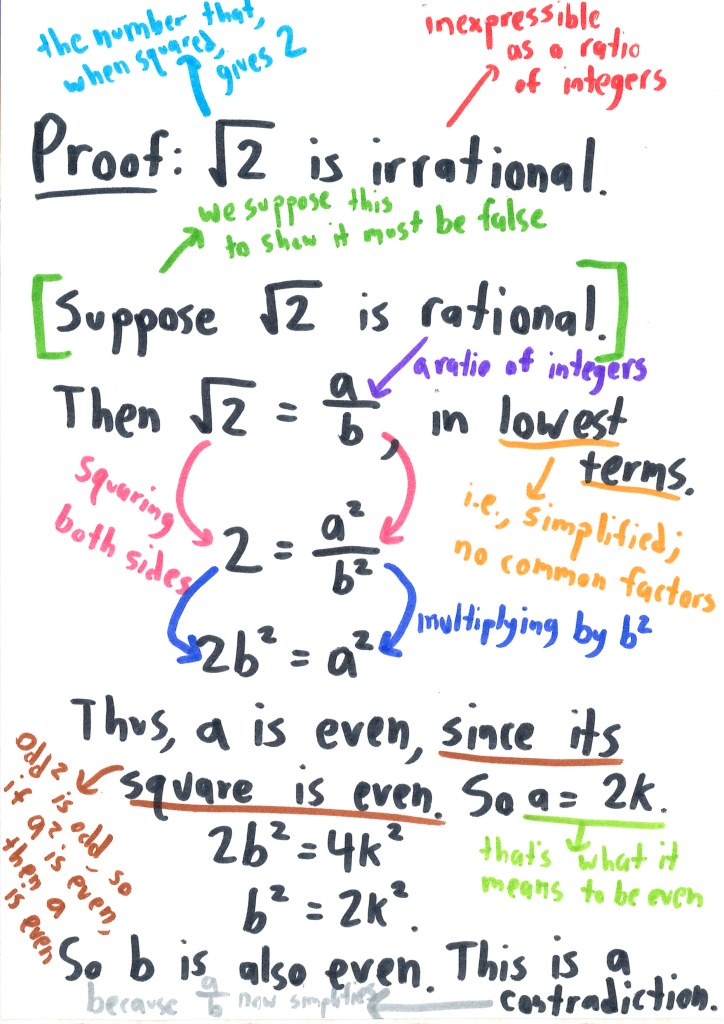
\includegraphics[width=0.5\textwidth]{media/read-with-pencil.jpg}
  \\ \scriptsize Image from~\cite{img:read_with_pencil}
\end{center}
You are not God.
You cannot keep everything in your head.\footnote{See also
	\url{https://blog.evanchen.cc/2015/03/14/writing/} and the source above.}
If you've printed out a hard copy, then write in the margins.
If you're trying to save paper,
grab a notebook or something along with the ride.
Somehow, some way, make sure you can write. Thanks.

\section{Further Reading}
The appendix \Cref{ch:refs} contains a list of resources I like,
and explanations of pedagogical choices that I made for each chapter.
I encourage you to check it out.

In particular, this is where you should go for further reading!
There are some topics that should be covered in the Napkin,
but are not, due to my own ignorance or laziness.
The references provided in this appendix should hopefully help partially
atone for my omissions.

\section{Why Are There Two Maths Sections?}
You might have noticed that this book has two separate sections on mathematics.
That's because many people, at least according to their own (often misguided)
opinion, \emph{do not like maths}. Hence, I have decided to separate into two
distinct sections those portions of mathematics I consider \emph{absolutely
  essential} and those which are required only for certain applications or
fields, or for further studies in certain areas.


% I DON'T want to reset the page number for mainmatter,
% so save it to restore later
\cleardoublepage{}
\newcounter{temppage}
\setcounter{temppage}{\value{page}}
\mainmatter{}
\setcounter{page}{\value{temppage}}

\tableofcontents

\Opensolutionfile{tex/backmatter/all-hints}
\Opensolutionfile{tex/backmatter/all-solns}

\part{Starting Out}\label{part:startout}
\parttoc{}
\setcounter{chapter}{-1} % sales pitch should be chapter 0
\chapter{Sales pitches}\label{ch:sales}
\newcommand{\pitch}[1]{\ii[\textsf{\color{blue}\ref{#1}}.] \textsf{\color{blue} \textbf{\nameref{#1}.}} \\[1ex]} % for now. . .
\newcommand{\buzzword}[1]{\textbf{\color{green!40!black} #1}}

This chapter contains a pitch for each part,
to help you decide what you want to read
and to elaborate more on how they are interconnected.

% TODO:
%For convenience, here is again the dependency plot
%that appeared in the frontmatter.
%\input{tex/frontmatter/digraph}

\section{Mathematics}
\begin{itemize}
  \pitch{part:foundations}
  This is the fundamental amount of mathematics required to understand
  anything in this book. Which is not a lot, really. It largely concerns
  basic set theory and the nature of logical statements.

  \pitch{part:maths}
  This contains all further mathematics you are likely to encounter over the
  course of a computer science degree. Some of it (such as linear algebra) may
  be extremely general and applicable to many different areas, some of it (such
  as numerical analysis) may be essential to how computers work on a fundamental
  level.
  Other parts (such as probability or number theory) may be specific to certain
  applications only.
\end{itemize}

\section{Theory}
\begin{itemize}
  \pitch{part:theoretical}
  This section concerns itself with what it means to
  \emph{compute} anything at all, what a computer even is, in the theoretical
  sense, what it can and --- perhaps more importantly --- \emph{cannot} compute.
  In this, we treat computation not as a list of instructions or an interaction
  of hardware components, but as a theoretical process that follows certain
  formalisms and rules.

  We begin with finite automata and their languages --- the regular expressions,
  before moving on to context-free grammars and push-down automata and
  finally into Turing machines, which model all of what a real computer
  can do.

  We will also delve into proofs
  of the correctness of such machines, systems verification, formal process
  algebra and more.

  \pitch{part:dsa}
  This is where we move away from the question of
  \emph{whether} something can be computed and instead ask ourselves
  \emph{how} and \emph{how well} it can be computed, as well as how to
  actually do so in the most efficient way possible.

  We begin with the basics of how data may be represented in memory, or in a more
  abstract context, using various data structures.

  Then we'll introduce algorithms to traverse, sort, search and manage these
  structures, all while measuring how efficient various approaches and
  algorithms are in terms of time and memory required.

  We analyze why, how and in which context certain approaches are more efficient
  than others and how you may perform such analysis on your own, for any
  algorithm, theoretical or implemented.

  \pitch{part:architecture}
  At its core, a computer is really just an electronic machine, in which
  electrons flow in a certain way to react to inputs and produce outputs
  via their currents.

  In this section, we concern ourselves with how to construct a CPU, how
  memory is structured and accessed, and how performance is impacted by
  both physical and logical design, as well as their interactions.

  We will also briefly introduce machine language and assembly code,
  and cover how digital files get loaded into the CPU and transformed into
  physical effects, as well as how modern assembly techniques like pipelining
  may improve performance.

  In essence, this section covers the intersection of, and various means of
  interfacing between hardware and software.

  \pitch{part:quantum}
  What happens when a computer operates by the laws of quantum physics?
  Here, we shall journey into the strange world of quantum computation, where
  bits may be zero or one\dots or something in between.
  Where reading data may be a write-operation and all notions of
  \emph{parallelism} fundamentally change meaning.

  We begin by introducing the required physics --- just enough to understand
  what \emph{superposition}, \emph{entanglement} and \emph{interference} are,
  before building up the mathematics required to represent quantum states.

  The core of this part of the book focuses on quantum circuits and how they
  are used to model and design algorithms for quantum computers. We will solve
  a number of conventionally \emph{hard} problems, such as prime factorization
  (using Shor's algorithm) or searching (using Grover's algorithm) in a
  radically more efficient manner than conventional computers would allow.
\end{itemize}

\section{Software Development}
\begin{itemize}
  \pitch{part:programming}
  Programming is the primary tool used to \emph{make computers do things}.
  In this chapter, we will cover the basics of what types of languages are used,
  which paradigms they are used in and what styles we choose and why. Here, we
  cover all aspects of programming from low-level to abstract.

  We begin with imperative programming: variables, control-flow, loops, state
  and mutation. Then we move on to object-oriented programming, and see how
  encapsulation, inheritance and polymorphism affect larger software systems.

  Beyond that, we will cover the functional programming paradigm, in which
  code consists of pure functions, in the mathematical sense and side-effects
  are avoided, as well as logic programming, where computation turns into a
  matter of proof and constraint satisfaction.

  We will finish this part with practical tips on how to learn the process of
  programming itself, new programming languages and how to work in unfamiliar
  paradigms, before giving a list of useful and educational practice problems
  to learn or master a variety of subjects, from a programming language itself
  to various highly theoretical or practical applications covered in this very
  book.

  \pitch{part:engineering}
  Software engineering is all the parts of the development process of software
  that \emph{aren't} programming. From designing software to meet requirements,
  to planning the development of large projects and testing, maintaining and
  managing existing software.

  We begin with core design patterns, which serve as reusable solutions to
  common architectural problems, then cover how to gather requirements,
  write specifications, perform version control and coordinate changes safely
  over time, even across large groups.

  Testing and debugging will be a major theme: how do you ensure that software
  does precisely what you want it to do, and keeps doing so as you extend it?
  We will also cover agile methods, project management best-practices and DevOps
  methodology --- covering deployment, monitoring and CI/CD.\@

  \pitch{part:hci}
  Good software should not just be functional, technically solving a problem.
  It should also be intuitively usable. This part is about how to properly
  design systems for human use, ensuring that our intended user base may
  understand, control and benefit from the clever algorithms and programs we
  come up with.

  We begin with principles of usability and accessibility: how to create
  interfaces that are clear, efficient and inclusive, before exploring visual
  design, interaction modeling and feedback loops, using desktop, mobile and
  web-interfaces as examples.

  We also study how to evaluate an interface, process user-feedback and other
  metrics, as well as how to perform proper user testing and iterative
  refinement.
\end{itemize}

\section{Systems and Infrastructure}
\begin{itemize}
  \pitch{part:compilers}
  We've heard about assembly at this point.
  But how does high-level code, utilizing complex abstractions, turn into
  byte-wise instructions for our CPU\@?

  We begin with lexical analysis (turning text into abstract tokens),
  parsing (representing the structure of a program), and intermediate
  representations, before exploring various optimizations that compilers
  employ to make code run faster without changing its meaning, and finally
  to code-generation, in which assembly instructions are emitted for a processor
  to physically execute.

  We also delve into type systems that can catch errors before the code is ever
  executed, and runtime systems that manage such things as memory, garbage
  collection and function calls.

  Building a compiler is a process that involves theory, algorithms and
  low-level systems architecture. After reading this part of the book, you
  should have understood a core part of every programming language, and perhaps
  even be able to create your own.

  \pitch{part:db}
  As we store more data than could (or should) fit into a single data structure,
  we need a database. This part of the book introduces the theory and practice
  of managing, organizing, structuring and maintaining data at scale.

  We begin with the concept of relational databases and SQL, the Standard Query
  Language used to access and modify structured data. Then we will study how to
  design schemas, normalize tables and use Entity-Relation diagrams to model
  real-world domains.

  Transactions, indexing and concurrency follow --- giving you the tools to
  understand \emph{how} databases keep data consistent across failures, respond
  quickly to any query and scale to several million users in the most extreme
  cases.

  Towards the end of this section, we then cover NoSQL models and how one may
  structure data in other manners, as well as the motivation for doing so.

  \pitch{part:os}
  How does a CPU decide what to run? How are multiple processes running at once,
  without interfering with each other? How is memory allocated without conflicts
  and why can two programs seemingly access the same addresses?

  Here, we answer those questions and more, by delving into the design of
  operating systems. We will study the nature of processes and threads, CPU
  and I/O scheduling, memory management, file systems and virtualization.

  We will explore how operating systems enforce the boundaries between
  processes while allowing for inter-process communication, and how they
  optimize performance on modern hardware. We will also cover classic
  problems like deadlocks, race-conditions and resource contention, as well
  as how they are solved in theory and practice.

  \pitch{part:distributed}
  Not all computer processes run on a single machine.
  This part shall cover those systems which run \emph{in parallel}, whether
  that is on multiple processor cores, or across multiple physically separate
  machines.

  We begin by covering concurrency and multithreading: how one designs a program
  that can do multiple things at once, safely. Then we move to distributed
  algorithms and the concepts of consensus, fault-tolerance and coordination
  across unreliable networks (which are all networks).

  We study protocols like gossip and Paxos, as well as systems like MapReduce
  and Spark, and explore modern architectures for compute clusters, cloud
  computing and data processing at scale.

  \pitch{part:networking}
  Computers are more useful when connected to other computers.
  Networking is how they are connected, and in this part of the book we will
  cover how that works, from the physical signals traveling through wires up to
  the final application.

  We begin with the OSI model and TCP/IP protocol, laying out the architecture
  of the internet. Then we look at how data is addressed, routed and
  transmitted, and how sockets allow programs to communicate with one another.

  We'll also cover common protocols (like HTTP, HTTPS, FTP, DNS), network
  performance analysis and network-related security concerns and threats
  and their mitigations.

  \pitch{part:cybersec}
  Once your computer connects to others --- or to an untrusted user --- security
  is no longer optional. Here, we cover how systems may be attacked by a
  malicious actor and how they may be defended against such attacks.

  We begin by covering cryptography: how data is encrypted and signed and
  identities are verified, before exploring authentication systems, common
  vulnerabilities (like overflow and injection attacks), thread modeling and
  security policies.

  Later chapters will cover blockchains, secure communication protocols and the
  human factors of digital security.
\end{itemize}

\section{Applications}
\begin{itemize}
  \pitch{part:ai}
  How do computers learn from data, recognize patterns or reason about uncertain
  scenarios? This part of the book shall introduce the tools and ideas behind
  machine learning and AI\@.

  We begin with statistical learning --- fitting models to given data --- and
  proceed through classification, clustering and regression algorithms using
  neural networks and random forests.

  Towards the end of this part, we explore the theory behind large language
  models and natural language processing, to see how modern generative AI
  creates texts or summarizes documents.

  \pitch{part:graphics}
  How do you turn data into images? How do you simulate the appearance of light,
  color and motion on a screen? In this section, we use computation to generate
  and manipulate visual scenes.

  We will cover the core rendering pipeline, from modeling geometry to
  projecting a 2D or 3D scene onto a screen. We will introduce shaders,
  ray-tracing and texture mapping, as well as covering human perception,
  color theory and visual design.
  In later chapters, we will touch on augmented and virtual reality.

  \pitch{part:bioinformatics}
  Life sciences --- meaning biology, chemistry and related fields --- have
  become a data science of their own. In this part, we explore how computation
  may help us model the properties of substances and the processes of their
  interactions, as well as help us understand life itself.

  We begin with sequence analysis: how to align DNA, determine similarity or
  distance between two biological sequences, find motifs and compare individuals and
  species based on their DNA\@.

  We will then explore computer-based structure analysis and chemoinformatics,
  in which computers may help design drugs, interpret experiments and uncover
  the rules that govern complex chemical interactions.

  Finally, we will cover computational systems biology, in which we use methods
  of computer science to interpret large datasets regarding biological and
  medical applications.
\end{itemize}


\part{Mathematical Foundations}\label{part:foundations}
\parttoc{}
\chapter{Mathematical Statements and Formal Logic}\label{ch:statements}
\section{Definition of a Statement}

\begin{definition}
  A statement (in the mathematical or logical sense) can always be sensibly
  assigned a truth value, namely ``true'' or ``false'' (also represented as 1/0).
  Statements the truth of which we have accepted by proof may be called
  \emph{theorem}, \emph{lemma}, \emph{proposition} or \emph{corollary},
  depending on their importance.
  Statements which we assume to be true by definition alone are called
  \emph{axioms}.
\end{definition}

\begin{example}
  [Examples and counterexamples of mathematical statements]
  \begin{itemize}
    \leavevmode
    \ii{} ``\(1+2=3\)'' is a true statement.
    \ii{} ``Squares of natural numbers may be negative'' is a false statement
          (but \emph{it is} a statement!).
    \ii{} ``x+1=2'' only becomes a mathematical statement when we choose a
          particular value of \(x\), or otherwise add something along the lines
          of ``there exists a number x, such that''. On its own, it is
          not a statement.
   \ii{} ``This statement is false'' is not a mathematical statement at all,
          since it can be neither true nor false.
  \end{itemize}
\end{example}

\begin{exercise}
  [Statements]
  Which of the following are \emph{mathematical statements}?
  \begin{enumerate}
    \ii{\(3+5=8\)}
    \ii{\(12-2=15\)}
    \ii{\(x+3=10\)}
    \ii{Let \(x\) be an integer.}
    \ii{There exists a prime number greater than \(1000\).}
    \ii{This sentence is false.}
    \ii{Every even number greater than \(2\) is the sum of two primes.}
  \end{enumerate}

  \begin{hint}
    Any mathematical statement must be either definitely true or definitely
    false. But you don't necessarily have to \emph{know} whether it is true or
    false. There exist statements the truth of which is yet to be discovered.
  \end{hint}

  \begin{sol}
    \begin{enumerate}
      \ii{\(3+5=8\)} We know for a fact that this is true. So it is a statement.
      \ii{\(12-2=15\)} We know for a fact that this is false. So it is a statement.
      \ii{\(x+3=10\)} This is not a fully specified statement. It may be true or
            false, depending on the value of \(x\). On its own, it is not a statement.
      \ii{Let \(x\) be an integer.} This is a declaration or an instruction. Not a
            statement in the mathematical sense. It has no truth value associated
            with it.
      \ii{There exists a prime number greater than \(1000\).} This is true. So it
            is a statement.
      \ii{``This sentence is false.''} This is a paradox. It cannot be
            true, nor can it be false. Hence, it is not a valid statement.
      \ii{Every even number greater than \(2\) is the sum of two primes.}
            This is a statement. We do not know if it is true (it's a famous
            unsolved problem, in fact!), but we know for a fact that it must be
            either true or false. So it satisfies the definition of what a
            statement is.
    \end{enumerate}
  \end{sol}
\end{exercise}

\section{Logical Operations}
Once we have constructed a logical statement, we may apply operations to it.
Logical statements may be combined freely with these operators, always producing
other logical statements. We define the following common operations by their
truth tables:

{ % Block for local table labeling
\captionsetup[table]{labelformat=empty, hypcap=false}

\begin{tcolorbox}[colframe=gray!80, colback=white, boxrule=0.4pt, top=4pt, bottom=4pt]
  \begin{minipage}[t]{0.32\textwidth}
    \centering
    \vspace{-10pt} % reduce space above caption
    \captionof{table}{Negation \(\neg\) \\(\emph{not A})}
    \vspace{10pt}  % add space between caption and table
    \begin{tabular}{c c}
      \(A\) & \(\neg A\) \\
      \midrule
      0 & 1 \\
      1 & 0
    \end{tabular}
  \end{minipage}
  \hfill
  \begin{minipage}[t]{0.32\textwidth}
    \centering
    \vspace{-10pt}
    \captionof{table}{Conjunction \(\land\) \\(\emph{A and B})}
    \vspace{3pt}
    \begin{tabular}{cc c}
      \(A\) & \(B\) & \(A \land B\)\\
      \midrule
      0 & 0 & 0 \\
      0 & 1 & 0 \\
      1 & 0 & 0 \\
      1 & 1 & 1 \\
    \end{tabular}
  \end{minipage}
  \hfill
  \begin{minipage}[t]{0.32\textwidth}
    \centering
    \vspace{-10pt}
    \captionof{table}{Disjunction \(\lor\) \\(\emph{A or B})}
    \vspace{3pt}
    \begin{tabular}{cc c}
      \(A\) & \(B\) & \(A \land B\)\\
      \midrule
      0 & 0 & 0 \\
      0 & 1 & 1 \\
      1 & 0 & 1 \\
      1 & 1 & 1 \\
    \end{tabular}
  \end{minipage}
\end{tcolorbox}

\begin{remark}
  These tables read (for two example rows) as follows: \\
  If logical statement \(A\) is true, then \(\neg A\) is a logical statement
  meaning \emph{not A} and it is false.\\
  If logical statement \(A\) is false and logical statement \(B\)
  is false, then \(A \land B\) is a logical statement meaning
  \emph{A and B} and it is false.
\end{remark}

Perhaps somewhat more interesting for our purposes are the following logical
operations

\begin{tcolorbox}[colframe=gray!80, colback=white, boxrule=0.4pt, top=4pt, bottom=4pt]
  \begin{minipage}[t]{0.48\textwidth}
    \centering
    \vspace{-10pt}
    \captionof{table}{Implication \(\Rightarrow\) \\(\emph{if A then B})}
    \vspace{3pt}
    \begin{tabular}{cc c}
      \(A\) & \(B\) & \(A \Rightarrow B\)\\
      \midrule
      0 & 0 & 1 \\
      0 & 1 & 1 \\
      1 & 0 & 0 \\
      1 & 1 & 1 \\
    \end{tabular}
  \end{minipage}
  \hfill
  \begin{minipage}[t]{0.48\textwidth}
    \centering
    \vspace{-10pt}
    \captionof{table}{Equivalence \(\Leftrightarrow\) \\
      (\emph{A is equivalent to B})}
    \vspace{3pt}
    \begin{tabular}{cc c}
      \(A\) & \(B\) & \(A \Leftrightarrow B\)\\
      \midrule
      0 & 0 & 1 \\
      0 & 1 & 0 \\
      1 & 0 & 0 \\
      1 & 1 & 1 \\
    \end{tabular}
  \end{minipage}
\end{tcolorbox}

Which are often used to express the flow of formal proofs.
\(A \Rightarrow B\) reads as \emph{if A then B}. Meaning that if statement \(A\)
is true, \(B\) must always also be true. Note that this makes no statement
about the value of \(B\) in the case where \(A\) is false.
\(A \Leftrightarrow B\) on the other hand reads as \emph{A if and only if B}.
Either both are true, or neither are. In some sense, they are fundamentally the
same statement put in different terms.

A less common form of notation is \(A \Leftarrow B\) which simply reads as
\emph{if B then A} and is equivalent to \(B \Rightarrow A\).

Finally, there is the operation on which most low-level computer operations are
based:

\begin{tcolorbox}[colframe=gray!80, colback=white, boxrule=0.4pt, top=4pt, bottom=4pt]
  \begin{minipage}[t]{\textwidth}
    \centering
    \vspace{-10pt}
    \captionof{table}{Exclusive or \(\xor\) \\(\emph{either A or B})}
    \vspace{3pt}
    \begin{tabular}{cc c}
      \(A\) & \(B\) & \(A \xor B\)\\
      \midrule
      0 & 0 & 0 \\
      0 & 1 & 1 \\
      1 & 0 & 1 \\
      1 & 1 & 0 \\
    \end{tabular}
  \end{minipage}
\end{tcolorbox}
}

\subsection{Compound Statements}
We may freely combine logical statements using any of these operations, always
creating new logical statements at each step. For instance,
\begin{example}
  [Compound statements]
  \((A \lor B) \Rightarrow C\)
  \hfill
  \((A \land B) \Leftrightarrow C\)
  \hfill
  \(A \lor (B \land C)\)
  \hfill
  \(A \land (B \Leftarrow C)\)
\end{example}

are all logical statements that may be true or false, depending on the values of
\(A, B, C\).
I have used parentheses to clarify the intended order of operations here, which
is often done for simplicity. However, just like with arithmetic operations
(\(+, -, \times, \div\)), precedence rules still exist:
\begin{itemize}
  \ii{} Negation \(\neg\) is evaluated first, followed by
  \ii{} Conjunction \(\land\)
  \ii{} Disjunction \(\lor\)
  \ii{} Implication \(\Rightarrow\) and
  \ii{} Equivalence \(\Leftrightarrow\)
\end{itemize}

\begin{exercise}
  [Logical Operator Precedence]
  Using parentheses, make the order of operations explicit, without changing the
  meaning of the statement.\\
  \(\neg A \lor B \land C \Rightarrow D\)

  \begin{sol}
    \(((\neg A) \lor (B \land C)) \Rightarrow D\)
  \end{sol}
\end{exercise}

\begin{example}
  [Signifying the precedence of logical operators]
  Consider the compound logical statement:\\
  \begin{center}
    \(\neg A \lor A \land B\)
  \end{center}
  It reads as follows: Either \(A\) is false, or \(B\) and \(C\) are both true.

  This is correctly evaluated by first negating \(A\), then evaluating
  \(B \land C\), then the logical or combining both.
\end{example}

\begin{exercise}
  [Logically Evaluating Statements]
  Let \(A=0, B=1, C=1\). Evaluate the following statement:\\
  \begin{center}
    \((\neg A \lor B) \Leftrightarrow (B \land C)\)
  \end{center}

  \begin{sol}
    \begin{align*}
      (\neg A \lor B) &\Leftrightarrow (B \land C)\\
      (\neg 0 \lor 1) &\Leftrightarrow (1 \land 1)\\
      (1 \lor 1) &\Leftrightarrow (1)\\
      1 &\Leftrightarrow 1\\
      &\ \, 1
    \end{align*}
  \end{sol}
\end{exercise}

\section{Tautologies}

We can, using these methods, construct statements that are always true.
A simple example of this might be \(A \lor \neg A\) or \(A \Rightarrow A\),
where \(A\) is any statement. Similarly, we may also construct statements that
must always be false, such as \(A \land \neg A\) or \(A \Leftrightarrow \neg A\).

We call statements that are always true by nature \emph{tautologies} and
those that are always false \emph{contradictions}. They are denoted by the
symbols \(\top\) and \(\bot\), respectively.

\begin{exercise}
  [Tautology and Contradiction]
  Are the following statements a tautology, a contradiction or neither?
  Can any statement be both?\\
  \((A \Rightarrow B) \Leftrightarrow (\neg A \lor B)\)\\
  \((A \xor B) \Leftrightarrow \neg (A \Leftrightarrow B)\)

  \begin{sol}
    The statements are tautologies. They expresses common logical identities, namely
    that \(A \Rightarrow B\) is the same statement as \(\neg A \lor B\)
    and \(A \xor B\) is the exact opposite statement as \(A \Leftrightarrow B\).\\
    No statement can be both tautology and contradiction, since that would
    require it to be true and false simultaneously. This would contradict our
    definition of what a logical statement is.
  \end{sol}
\end{exercise}

% TODO: Most of these should probably be questions or exercises, not problems.
\section{\problemhead}
\begin{problem}
  [Truth tables]
  Construct the truth-table for the following statement:\\
  \begin{center}
    \(A \Rightarrow (B \lor \neg C)\)
  \end{center}

  \begin{hint}
    First compute the truth tables for the intermediate values of \(\neg C\) and
    \(B \lor \neg C\) in their own columns.
  \end{hint}

  \begin{sol}
    \begin{tabular}{ccc cc c}
      \(A\) & \(B\) & \(C\) & \(\neg C\) & \(B \lor \neg C\) &
      \(A \Rightarrow (B \lor \neg C)\)\\
      \midrule
      0 & 0 & 0 & 1 & 1 & 1\\
      0 & 0 & 1 & 0 & 0 & 1\\
      0 & 1 & 0 & 1 & 1 & 1\\
      0 & 1 & 1 & 0 & 1 & 1\\
      1 & 0 & 0 & 1 & 1 & 1\\
      1 & 0 & 1 & 0 & 0 & 0\\
      1 & 1 & 0 & 1 & 1 & 1\\
      1 & 1 & 1 & 0 & 1 & 1\\
    \end{tabular}
  \end{sol}
\end{problem}

% \include{tex/foundations/boolean_algebra}
% \include{tex/foundations/proof_techniques}
\chapter{Sets}\label{ch:sets}
\section{Definition}
\begin{definition}
  A set is an unordered collection of distinct objects.
  We write sets surrounded by curly braces, with each element
  separated from the others by a comma.
\end{definition}
\begin{example}
  [A set]
  For example: \(A = \{1, 2, 3\}\) is the set
  containing the numbers one, two and three.
\end{example}

\section{Key Properties}
\begin{itemize}
  \ii{\textbf{Unordered:}} sets are unordered. That is, \(\{1,2,3\}=\{3,2,1\}\),
  because they contain the same elements, only in a different order.
  \ii{\textbf{No duplicates:}} sets only contain each element at most once.
  That is, \(\{1,2,3\}=\{1,2,2,3,3,3\}\), because they contain the same
  elements, only differing in \emph{how often} they occur.
\end{itemize}

\section{Membership}
A set may \emph{contain elements}.
To express that a given element \(x\) is contained within a set \(A\),
we write \(x \in A\). To express that an element \(y\) is \emph{not} contained
within a set \(A\), we write \(y \notin A\).

Two sets \(A, B\) are considered equal, precisely when
\((x \in A) \Leftrightarrow (x \in B)\) for all objects \(x\).

There exists a set that has no elements at all. It is called \emph{the empty
  set} and usually denoted as \(\emptyset\).
\(x \in \emptyset\) is a false statement for every possible object \(x\),
whereas \(x \notin \emptyset\) is true for every object \(x\).

\section{Subsets and Powersets}

Let \(A, B\) be sets. Then \(A\) is called a \emph{subset} of \(B\) if and only if
every element of \(A\) is also in \(B\). We express this by the notation
\(A \subseteq B\). We further introduce the notation \(A \subsetneq B\) to mean
\((A \subseteq B) \land (A \neq B)\). In this case, \(A\) is called a \emph{proper
  subset} of \(B\).

We may equivalently state that \(B\) is a \emph{superset} of \(A\), and express
this as \(B \supseteq A\), or \(B \supsetneq A\) if they are not equal.

If \(A\) is a set, then the set of all subsets of \(A\) is called its
\emph{powerset} \(\PP(A)\).

\begin{example}
  [Subsets, supersets]
  \begin{itemize}
    \leavevmode
    \ii{The empty set is a subset of every set}:
          \(\emptyset \subseteq A\) for every set \(A\)
    \ii{Every non-empty set is a \emph{proper superset} of the empty set}:
          \(A \supsetneq \emptyset\) for every set \(A, A \neq \emptyset\)
    \ii{} \(\{1,2,3\} \subseteq \{1,2,3,4,5\}\)
    \ii{} \(a \in A \Leftrightarrow \{a\} \subseteq A\), though the set containing an object \emph{is a
          different thing than the object itself}
    \ii{} if \(A = \{1,2,3\}\), then
          \(\PP(A) = \{\emptyset, \{1\}, \{2\}, \{3\}, \{1,2\}, \{1,3\}, \{2,3\}, \{1,2,3\}\}\)
  \end{itemize}
\end{example}

\section{Quantifiers}

Often times, we would want to express a statement that holds \emph{for every
  element} of a set, or at least for \emph{some elements}.
Or perhaps, we might want to state that a statement is true only for
 \emph{exactly one element} within a set. That's what quantifiers do.

\begin{tcolorbox}[colframe=gray!80, colback=white, boxrule=0.4pt, top=4pt, bottom=4pt]
  \begin{minipage}[t]{\textwidth}
    \centering
    \vspace{-10pt}
    \captionof{table}{Logical Quantifiers}
    \vspace{3pt}
    \begin{tabular}{cc}
      \(\forall\) & ``for all''\\
      \(\exists\) & ``there exists at least one (but possibly many)''\\
      \(\exists!\) & ``there exists \emph{exactly} one''
    \end{tabular}
  \end{minipage}
\end{tcolorbox}

 \begin{example}
   [Quantifiers]
 Consider, for instance, the statement: \emph{``Every natural number --- including
 zero ---  may be expressed as the sum of two natural numbers''}.

We would express this using the following notation:
\begin{center}
  \(\forall x \in \NN_0 : x = y + z \qquad y,z\in\NN_0\)
\end{center}

And usually mean to imply that this is a true statement, unless specified otherwise.
\end{example}

\section{Describing Sets}
Sets may be described in a number of ways.
The simplest method --- which we have used thus far --- is by simply listing out
all elements within the set.
However, this is only convenient for small, and only possible at all for
\emph{finite} sets.
Infinite sets exist, however, and must be described using different means.
Consider, for instance, the set \(\NN_{0} = \{0,1,2,3,4,5,\dots\}\),
which contains all \emph{natural numbers}, starting at zero.
From this, we may construct further sets, such as
\(\ZZ = \{x-y \mid x, y \in \NN_0\}\), which is the set of all
\emph{integers}.
\begin{remark}
  This notation reads as ``Let \(\ZZ\) be the set containing all differences
  x-y, where x and y are natural numbers'', or more concisely ``Let \(\ZZ\)
  be the set of all possible differences of natural numbers''. It still includes
  all natural numbers, since \(x - 0 \in \ZZ \forall x \in \NN_0\), so we may
  note that \(\NN_0 \subseteq \ZZ\), but it also contains negative integers, since \(0 - x\)
  is similarly contained.
  So we may note that \(\NN_0 \subseteq \ZZ\).
\end{remark}

From these, we can then further construct the set
\(\QQ = \{\frac{x}{y} \mid x,y \in \ZZ, y \neq 0\}\) of all
\emph{rational numbers}.

Sets are central to virtually all branches of mathematics and theoretical
computer science. They provide the language in which most other concepts are
defined and formalized.

We note at this point, that not every \emph{description} of a set creates
another valid set: consider for instance \(\{A \mid A \notin A\}\), or \emph{the
set of all sets that do not contain themselves}. Such a set cannot exist, as its
construction inevitably leads to a paradox: should it contain itself?

\section{Commonly Used Sets}
Commonly used sets include:
\begin{itemize}
  \ii{\(\NN\):} The set of all \emph{natural numbers}, meaning all the positive integers
        you'd use to count things.
\begin{remark}
  The set \(\NN\) is sometimes understood to include \(0\), sometimes understood
  to not include it. This ambiguity is annoying.
  In this book, I shall always explicitly use \(\NN_{0}\) to denote the set of
  natural numbers \emph{including} zero and \(\NN^{*}\) to denote the set of
  natural numbers \emph{without} zero.
\end{remark}
  \ii{\(\ZZ\):} The set of all \emph{integers}, including the negative integers.
  \ii{\(\QQ\)} The set of all \emph{rational numbers}, which are the ratios of integers,
        ie.\ fractions.
  \ii{\(\RR\):} The set of all \emph{real numbers}, including all those that cannot be
        expressed as fractions, such as \(\sqrt{2}, \pi\) or \(e\)
  \ii{\(\CC\)} The set of all \emph{complex numbers}
\end{itemize}

Each of these sets is also a \emph{proper subset} of the next, that is
\begin{align*}
  \NN \subsetneq \ZZ \subsetneq \QQ \subsetneq \RR \subsetneq \CC
\end{align*}

\section{Set Operations}
Much like logical statements, sets have their own associated operations.
In the following list, let \(A, B\) be any two sets.
\begin{itemize}
  \ii{\textbf{Intersection:}}
        \(A \cap B \defeq \{x \mid x \in A \land x \in B\}\)
  \ii{\textbf{Union:}}
        \(A \cup B \defeq \{x \mid x \in A \lor x \in B\}\)
  \ii{\textbf{Difference:}}
        \(A \setminus B \defeq \{x \mid x \in A \land x \notin B\}\)
  \ii{\textbf{Symmetric Difference:}}
        \(A \symdif B \defeq \{x \mid x \in A \xor x \in B\}\)
  \ii{\textbf{Cartesian Product:}}
        \(A \times B \defeq \{(x, y) \mid x \in A \land y \in B\}\)\\
        Where \((x,y)\) is the ordered pair of two elements, one each from \(A, B\).
\end{itemize}

\begin{example}
  [Set Operations]
  \begin{itemize}
    \leavevmode
    \ii{\(\NN^* = \NN_0 \setminus \{0\}\)}
    \ii{\(\RR \cap \ZZ = \ZZ\)}
    \ii{\(\RR^2 = \RR \times \RR = \{(x, y) \mid x, y \in \RR\}\)}
      \\is the set of all points in the flat plane, and more generally
    \ii{\(\RR^{n} = \RR \times \cdots \times \RR = \{(x_{1}, \ldots, x_{n}) \mid x_{i} \in \RR\}\)}
      \\is the set of all points in \(n\text{-dimensional}\) space.
\end{itemize}
\end{example}

\section{\problemhead}
\begin{problem}
  [Example Problem]
  Let \(A=\{0,1,2,3\}\). Is \(0 \in A\)?
  \begin{hint}
    Try reading the notation on sets.
  \end{hint}
  \begin{sol}
    Yes. Zero is an element of the set \(A\).
  \end{sol}
\end{problem}

\chapter{Tuples}\label{ch:tuples}
\section{Definition}
\begin{definition}
  A tuple is an ordered list of finitely many objects.
  We write tuples surrounded by parentheses, with each element
  separated from the others by a comma.
  A tuple containing \(n\) elements is called an \(n\text{-tuple}\).
  \(2\text{-tuples}\) are sometimes referred to as \emph{pairs} or \emph{ordered pairs}.
\end{definition}
\begin{example}
  [A tuple]
  For example: \((3, 2, 2, 1)\) is the tuple
  containing the numbers three, two, another copy of two,
  and one, in that specific order.
\end{example}

\section{Key Properties}
\begin{itemize}
  \ii{\textbf{Ordered:}} unlike sets, tuples are ordered. That is,
      \((1,2,3) \neq (3,2,1)\),
  because their elements appear in a different order.
  \ii{\textbf{Duplicates:}} tuples may contain elements more than once.
  That is, \((1,2,3) \neq (1,2,2,3,3,3)\), because they contain the same
  elements, but differ in \emph{how often} they occur.
  \ii{\textbf{Finite:}} unlike sets, tuples are always finite.
  They cannot contain an infinite number of elements.
\end{itemize}

\section{Tuple Comparison}
Two tuples \emph{of the same length} may be compared to each other using
\(=, \neq, <, \leq, >, \geq\).
Let \(a = (a_{0}, a_{1}, \dots, a_{n-1}), b = (b_{0}, b_{1}, \dots, b_{n-1})\) be
two tuples of length \(n\). We compare them using the following rules:

\subsection*{Equality}
\begin{itemize}
  \ii{\(a = b\):} if and only if \(\forall i \in \{0, 1, \dots, n-1\}: a_{i} = b_{i}\)
  \ii{\(a \neq b\):} if and only if \(\exists i \in \{0, 1, \dots, n-1\}: a_{i} \neq b_{i}\)
\end{itemize}

\subsection*{Lexicographic Ordering}
\begin{itemize}
  \ii{\(a < b\):} if and only if
        \(\exists k \in \{0, 1, \dots, n-1\}: \forall i < k: a_{i} = b_{i} \land a_{k} < b_{k}\)
  \ii{\(a \leq b\):} if and only if \(a < b \lor a = b\)
  \ii{\(a > b\):} if and only if
        \(\exists k \in \{0, 1, \dots, n-1\}: \forall i < k: a_{i} = b_{i} \land a_{k} > b_{k}\)
  \ii{\(a \geq b\):} if and only if \(a > b \lor a = b\)
\end{itemize}

This is called \emph{lexicographic} ordering, because it is precisely how a
lexicon (or a dictionary) orders words of the same length. Those with the
smaller initial letter are grouped first, then within that group we sort by the
second letter, and so on.

\begin{example}
  \begin{itemize}
    \leavevmode
    \ii{\((1,2,3) < (1,3,2)\)} because \(2 < 3\)
    \ii{\((1,2,3) \geq (1,2,3)\)} because they are equal.
    \ii{\((1,2,3) \neq (4,3,2,1)\)} are not equal, because they differ in
          length. We may not state that one is lesser or greater than the
          other, since they cannot be compared lexicographically.
  \end{itemize}
\end{example}


\section{Tuple Operations}
Much like logical statements, sets have their own associated operations.
In the following list, let \(A, B\) be any two sets.
\begin{itemize}
  \ii{\textbf{Element Access:}}
        \(t[n]\) refers to the \(n\text{-th}\) element of the tuple \(t\).
        We begin indexing elements at \(0\).
        For instance, \((1,2,3)[0] = 1\).
        \begin{remark}
          This is common notation in computer science, hence what we will use for
          purposes of this book. In mathematics, tuples are often indexed starting
          at \(1\) and element access is written is \(t_{n}\) or \(\pi_{n}(t)\).
        \end{remark}
  \ii{\textbf{Concatenation:}}
        \(t \circ u\) is the tuple which contains all elements of \(t\),
        followed by all elements of \(u\), where \(t,u\) are tuples.
  \ii{\textbf{Slicing:}}
        \(t[n:m] \mid m > n\) refers to the sub-tuple of length \(m-n\)
        containing all elements from the \(n\text{-th}\) up to the \(m\text{-th}\)
        element of \(t\), where the \(n\text{-th}\) element is included and the
        \(m\text{-th}\) element is not.
\end{itemize}

\begin{example}
  [Tuple Operations]
  \begin{itemize}
    \leavevmode
    \ii{\((8,12,82,-3,1)[2] = 82\)}
    \ii{\((1,2,3) \circ (4,5,6) = (1,2,3,4,5,6)\)}
    \ii{\((1,2,3,4,5,6)[2:5] = (3,4,5)\)}
\end{itemize}
\end{example}

% TODO: Add exercises and problems

% \chapter{Relations and Functions}\label{ch:functions}
\section{Relations}

\begin{definition}
  A (binary) relation \(R\) between two sets \(A, B\) is the 3-tuple of those
  two sets and any subset of their Cartesian product:
  \begin{align*}
    R \defeq (A, B, R') & \text{where} & R' \subseteq A \times B
  \end{align*}
  Which means that a relation between two sets is specified by those two sets
  and a set of pairs, in which the first element of each pair is from one set
  and the second element of each pair is from the other.

  The set \(A\) is then called the \emph{domain} of \(R\), and \(B\) is called
  its \emph{codomain}.
\end{definition}

A relation \emph{relates} objects from one set to objects from another (or possibly the same) set.

To express that a given pair is in such a relation, we may use
any of the following notations:
\begin{center}
\begin{tabular}{c c}
  \((a, b) \in R\) & \text{explicit set notation}\\
  \(R(a,b)\) & \text{prefix notation}\\
  \(a R b\) & \text{infix notation}
\end{tabular}
\end{center}

\begin{example}
  [Example of a relation]
  Let \(A=\NN, B=\NN\).
  Then \(<\) defines a relation from \(A\) to \(B\).\\
  For instance, \((1, 2) \in <\), or as this is more commonly denoted:
  \(1 < 2\). \\
  However, \((1, 0) \notin <\), meaning \( 1 \not< 0\).
\end{example}

\subsection{Uniqueness Properties}

A relation is called \emph{left-unique} if every element in its domain
is related to \emph{at most one} element of its codomain.
Similarly, a relation is called \emph{right-unique} if every element in the
codomain is related to \emph{at most one} element in the domain.

\subsection{Totality Properties}

A relation is called \emph{left-total} if every element in its domain
is related to \emph{at least one} element of its codomain.
Again, the term \emph{right-total} is used to describe the same idea
the other way around: every element of the codomain of a right-total relation
is related to \emph{at least one} element of its domain.

\section{Functions}

\begin{definition}
  A \emph{function} is a relation that is right-unique and left-total.
  We usually denote this as
  \begin{align*}
    f \colon A \to B
  \end{align*}
  meaning \emph{``Let \(f\) be a function from \(A\) to \(B\)''}.
  This means that \(f\) assigns each \(a \in A\) \emph{exactly one}
  \(b \in B\), though it may repeatedly assign the same elements of \(B\),
  or not assign some elements from \(B\) to any elements in \(A\) at all.
\end{definition}

\begin{definition}
  A function is called \emph{injective} if it is also left-unique, meaning it
  only assigns each element of the codomain \textit{at most once}.\\
  A function is called \emph{surjective} if it is also right-total, meaning it
  assigns each element of the codomain \textit{at least once}.\\
  A function is called \emph{bijective}, or \textit{one-to-one},
  if it is both injective and surjective.
\end{definition}

\begin{tikzpicture}

% Y coordinates for 3 points each side
\def\domainY{1.5,0,-1.5}
\def\codomainY{1.5,0,-1.5}

\ovalrelation{0cm}{0cm}
  {1.5,0,-1.5}
  {1.5,0,-1.5}
  {1/1,2/2}
  {A \textit{left-unique}, \textit{right-unique} relation}

\ovalrelation{7cm}{0cm}
  {1.5,0,-1.5}
  {1.5,0,-1.5}
  {1/1,1/2}
  {A \textit{left-unique} relation}

\ovalrelation{0cm}{-6cm}
  {1.5,0,-1.5}
  {1.5,0,-1.5}
  {1/1,2/2,2/3}
  {A \textit{left-unique}, \textit{right-total} relation}

\ovalrelation{7cm}{-6cm}
  {1.5,0,-1.5}
  {1.5,0,-1.5}
  {1/1,2/2,3/2}
  {\shortstack{A \textit{function} \\ (which is not injective or surjective)}}

\ovalrelation{0cm}{-12cm}
  {1.5,0,-1.5}
  {1.5,0,-1.5}
  {1/1,2/2,3/1}
  {An \textit{injective} function}

\ovalrelation{7cm}{-12cm}
  {1.5,0,-1.5}
  {1.5,0,-1.5}
  {1/1,2/1,3/2}
  {A \textit{surjective} function}

\ovalrelation{3.5cm}{-18cm}
  {1.5,0,-1.5}
  {1.5,0,-1.5}
  {1/1,2/2,3/3}
  {A \textit{bijective} function}

\end{tikzpicture}

% \include{tex/foundations/number_theory}

\part{Further Mathematics}\label{part:maths}
\parttoc{}
% \include{tex/maths/discrete_strutures}
% \include{tex/maths/linalg}
% (
%  \part{Linear Algebra}\label{part:linalg}
%  \parttoc{}
%  \include{tex/linalg/vector-space}
%  \include{tex/linalg/eigenvalues}
%  \include{tex/linalg/dual-trace}
%  \include{tex/linalg/dets}
%  \include{tex/linalg/inner-form}
%  \include{tex/linalg/fourier}
%  \include{tex/linalg/transpose}
% )
% \include{tex/maths/numerical_analysis}
% \include{tex/maths/calculus}
% (
%  \part{Calculus 101}\label{part:calc}
%  \parttoc{}
%  \include{tex/calculus/limits}
%  \include{tex/calculus/p-adic}
%  \include{tex/calculus/differentiate}
%  \include{tex/calculus/taylor}
%  \include{tex/calculus/integrate}
% )
% \include{tex/maths/combinatorics}
% \include{tex/maths/prob_stats}
% \include{tex/maths/number_theory}


\part{The Theory of Computation}\label{part:theoretical}
\parttoc{}
\chapter{Finite State Machines and Regular Expressions}\label{ch:fsm_regex}
\section{Finite Automata}

\begin{center}
  \begin{tikzpicture}
    \node[state, initial] (q0) {\(q_0\)};
    \node[state, accepting, right of=q0] (q1) {\(q_1\)};

    \path
      (q0) edge[bend left, above] node{a} (q1)
      (q1) edge[bend left, below] node{b} (q0);
  \end{tikzpicture}
\end{center}

\begin{tikzpicture}
  % States
  \node[state, initial] (q0) {\(q_0\)};
  \node[state, accepting, initial, right of=q0, xshift=3cm] (q1) {\(q_1\)};
  \node[state, below right of=q0] (q2) {\(q_2\)};
  \node[state, right of=q2] (q3) {\(q_3\)};
  \node[state, accepting, below of=q3] (q4) {\(q_4\)};
  \node[state, accepting, right of=q3, xshift=2cm] (q5) {\(q_5\)};

  % Transitions
  \path
    (q0) edge[above] node{a} (q2)
    (q1) edge[above] node{b} (q2)
    (q2) edge[loop below] node{b,c} ()
    (q2) edge[above] node{a} (q3)
    (q3) edge[below right] node{c} (q4)
    (q3) edge[bend left, above] node{a} (q5)
    (q4) edge[bend right, left] node{b} (q2)
    (q5) edge[loop right] node{a,b} ();
\end{tikzpicture}

% \include{tex/theory/pda_cfg}
% \include{tex/theory/turing_machines}
% \include{tex/theory/decidability}
% \include{tex/theory/complexity_classes}
% \include{tex/theory/buechi_omega_languages}
% \include{tex/theory/transistion_systems}
% \include{tex/theory/kripke_structures}
% \include{tex/theory/petri_nets}
% \include{tex/theory/higher_nets}
% \include{tex/theory/net_parallelism}
% \include{tex/theory/systems_verification}
% \include{tex/theory/temporal_logic}
% \include{tex/theory/model_checking}
% \include{tex/theory/process_algebra}


\part{Data Structures and Algorithms}\label{part:dsa}
\parttoc{}
% \include{tex/dsa/basic_structures}
% \include{tex/dsa/landau_symbols}
% \include{tex/dsa/sorting}
% \include{tex/dsa/searching}
% \include{tex/dsa/advanced_strutures}
% \include{tex/dsa/runtime_analysis}
% \include{tex/dsa/paradigms_approaches}
% \include{tex/dsa/graph_algorithms}


\part{Computer Architecture and Digital Logic}\label{part:architecture}
\parttoc{}
% \include{tex/architecture/gates_circuits}
% \include{tex/architecture/alu_registers_cycles}
% \include{tex/architecture/memory_hierarchy}
% \include{tex/architecture/assembly}
% \include{tex/architecture/pipelining_parallelism_performance}


\part{Quantum Computation}\label{part:quantum}
\parttoc{}
% \include{tex/quantum/phyics}
% \include{tex/quantum/qbits_foundations}
% \include{tex/quantum/vectors}
% \include{tex/quantum/circuits}
% \include{tex/quantum/shor}


\part{Programming}\label{part:programming}
\parttoc{}
% \include{tex/programming/imperative}
% \include{tex/programming/oop}
% \include{tex/programming/functional}
% \chapter{Mathematical Statements and Formal Logic}\label{ch:statements}
\section{Definition of a Statement}

\begin{definition}
  A statement (in the mathematical or logical sense) can always be sensibly
  assigned a truth value, namely ``true'' or ``false'' (also represented as 1/0).
  Statements the truth of which we have accepted by proof may be called
  \emph{theorem}, \emph{lemma}, \emph{proposition} or \emph{corollary},
  depending on their importance.
  Statements which we assume to be true by definition alone are called
  \emph{axioms}.
\end{definition}

\begin{example}
  [Examples and counterexamples of mathematical statements]
  \begin{itemize}
    \leavevmode
    \ii{} ``\(1+2=3\)'' is a true statement.
    \ii{} ``Squares of natural numbers may be negative'' is a false statement
          (but \emph{it is} a statement!).
    \ii{} ``x+1=2'' only becomes a mathematical statement when we choose a
          particular value of \(x\), or otherwise add something along the lines
          of ``there exists a number x, such that''. On its own, it is
          not a statement.
   \ii{} ``This statement is false'' is not a mathematical statement at all,
          since it can be neither true nor false.
  \end{itemize}
\end{example}

\begin{exercise}
  [Statements]
  Which of the following are \emph{mathematical statements}?
  \begin{enumerate}
    \ii{\(3+5=8\)}
    \ii{\(12-2=15\)}
    \ii{\(x+3=10\)}
    \ii{Let \(x\) be an integer.}
    \ii{There exists a prime number greater than \(1000\).}
    \ii{This sentence is false.}
    \ii{Every even number greater than \(2\) is the sum of two primes.}
  \end{enumerate}

  \begin{hint}
    Any mathematical statement must be either definitely true or definitely
    false. But you don't necessarily have to \emph{know} whether it is true or
    false. There exist statements the truth of which is yet to be discovered.
  \end{hint}

  \begin{sol}
    \begin{enumerate}
      \ii{\(3+5=8\)} We know for a fact that this is true. So it is a statement.
      \ii{\(12-2=15\)} We know for a fact that this is false. So it is a statement.
      \ii{\(x+3=10\)} This is not a fully specified statement. It may be true or
            false, depending on the value of \(x\). On its own, it is not a statement.
      \ii{Let \(x\) be an integer.} This is a declaration or an instruction. Not a
            statement in the mathematical sense. It has no truth value associated
            with it.
      \ii{There exists a prime number greater than \(1000\).} This is true. So it
            is a statement.
      \ii{``This sentence is false.''} This is a paradox. It cannot be
            true, nor can it be false. Hence, it is not a valid statement.
      \ii{Every even number greater than \(2\) is the sum of two primes.}
            This is a statement. We do not know if it is true (it's a famous
            unsolved problem, in fact!), but we know for a fact that it must be
            either true or false. So it satisfies the definition of what a
            statement is.
    \end{enumerate}
  \end{sol}
\end{exercise}

\section{Logical Operations}
Once we have constructed a logical statement, we may apply operations to it.
Logical statements may be combined freely with these operators, always producing
other logical statements. We define the following common operations by their
truth tables:

{ % Block for local table labeling
\captionsetup[table]{labelformat=empty, hypcap=false}

\begin{tcolorbox}[colframe=gray!80, colback=white, boxrule=0.4pt, top=4pt, bottom=4pt]
  \begin{minipage}[t]{0.32\textwidth}
    \centering
    \vspace{-10pt} % reduce space above caption
    \captionof{table}{Negation \(\neg\) \\(\emph{not A})}
    \vspace{10pt}  % add space between caption and table
    \begin{tabular}{c c}
      \(A\) & \(\neg A\) \\
      \midrule
      0 & 1 \\
      1 & 0
    \end{tabular}
  \end{minipage}
  \hfill
  \begin{minipage}[t]{0.32\textwidth}
    \centering
    \vspace{-10pt}
    \captionof{table}{Conjunction \(\land\) \\(\emph{A and B})}
    \vspace{3pt}
    \begin{tabular}{cc c}
      \(A\) & \(B\) & \(A \land B\)\\
      \midrule
      0 & 0 & 0 \\
      0 & 1 & 0 \\
      1 & 0 & 0 \\
      1 & 1 & 1 \\
    \end{tabular}
  \end{minipage}
  \hfill
  \begin{minipage}[t]{0.32\textwidth}
    \centering
    \vspace{-10pt}
    \captionof{table}{Disjunction \(\lor\) \\(\emph{A or B})}
    \vspace{3pt}
    \begin{tabular}{cc c}
      \(A\) & \(B\) & \(A \land B\)\\
      \midrule
      0 & 0 & 0 \\
      0 & 1 & 1 \\
      1 & 0 & 1 \\
      1 & 1 & 1 \\
    \end{tabular}
  \end{minipage}
\end{tcolorbox}

\begin{remark}
  These tables read (for two example rows) as follows: \\
  If logical statement \(A\) is true, then \(\neg A\) is a logical statement
  meaning \emph{not A} and it is false.\\
  If logical statement \(A\) is false and logical statement \(B\)
  is false, then \(A \land B\) is a logical statement meaning
  \emph{A and B} and it is false.
\end{remark}

Perhaps somewhat more interesting for our purposes are the following logical
operations

\begin{tcolorbox}[colframe=gray!80, colback=white, boxrule=0.4pt, top=4pt, bottom=4pt]
  \begin{minipage}[t]{0.48\textwidth}
    \centering
    \vspace{-10pt}
    \captionof{table}{Implication \(\Rightarrow\) \\(\emph{if A then B})}
    \vspace{3pt}
    \begin{tabular}{cc c}
      \(A\) & \(B\) & \(A \Rightarrow B\)\\
      \midrule
      0 & 0 & 1 \\
      0 & 1 & 1 \\
      1 & 0 & 0 \\
      1 & 1 & 1 \\
    \end{tabular}
  \end{minipage}
  \hfill
  \begin{minipage}[t]{0.48\textwidth}
    \centering
    \vspace{-10pt}
    \captionof{table}{Equivalence \(\Leftrightarrow\) \\
      (\emph{A is equivalent to B})}
    \vspace{3pt}
    \begin{tabular}{cc c}
      \(A\) & \(B\) & \(A \Leftrightarrow B\)\\
      \midrule
      0 & 0 & 1 \\
      0 & 1 & 0 \\
      1 & 0 & 0 \\
      1 & 1 & 1 \\
    \end{tabular}
  \end{minipage}
\end{tcolorbox}

Which are often used to express the flow of formal proofs.
\(A \Rightarrow B\) reads as \emph{if A then B}. Meaning that if statement \(A\)
is true, \(B\) must always also be true. Note that this makes no statement
about the value of \(B\) in the case where \(A\) is false.
\(A \Leftrightarrow B\) on the other hand reads as \emph{A if and only if B}.
Either both are true, or neither are. In some sense, they are fundamentally the
same statement put in different terms.

A less common form of notation is \(A \Leftarrow B\) which simply reads as
\emph{if B then A} and is equivalent to \(B \Rightarrow A\).

Finally, there is the operation on which most low-level computer operations are
based:

\begin{tcolorbox}[colframe=gray!80, colback=white, boxrule=0.4pt, top=4pt, bottom=4pt]
  \begin{minipage}[t]{\textwidth}
    \centering
    \vspace{-10pt}
    \captionof{table}{Exclusive or \(\xor\) \\(\emph{either A or B})}
    \vspace{3pt}
    \begin{tabular}{cc c}
      \(A\) & \(B\) & \(A \xor B\)\\
      \midrule
      0 & 0 & 0 \\
      0 & 1 & 1 \\
      1 & 0 & 1 \\
      1 & 1 & 0 \\
    \end{tabular}
  \end{minipage}
\end{tcolorbox}
}

\subsection{Compound Statements}
We may freely combine logical statements using any of these operations, always
creating new logical statements at each step. For instance,
\begin{example}
  [Compound statements]
  \((A \lor B) \Rightarrow C\)
  \hfill
  \((A \land B) \Leftrightarrow C\)
  \hfill
  \(A \lor (B \land C)\)
  \hfill
  \(A \land (B \Leftarrow C)\)
\end{example}

are all logical statements that may be true or false, depending on the values of
\(A, B, C\).
I have used parentheses to clarify the intended order of operations here, which
is often done for simplicity. However, just like with arithmetic operations
(\(+, -, \times, \div\)), precedence rules still exist:
\begin{itemize}
  \ii{} Negation \(\neg\) is evaluated first, followed by
  \ii{} Conjunction \(\land\)
  \ii{} Disjunction \(\lor\)
  \ii{} Implication \(\Rightarrow\) and
  \ii{} Equivalence \(\Leftrightarrow\)
\end{itemize}

\begin{exercise}
  [Logical Operator Precedence]
  Using parentheses, make the order of operations explicit, without changing the
  meaning of the statement.\\
  \(\neg A \lor B \land C \Rightarrow D\)

  \begin{sol}
    \(((\neg A) \lor (B \land C)) \Rightarrow D\)
  \end{sol}
\end{exercise}

\begin{example}
  [Signifying the precedence of logical operators]
  Consider the compound logical statement:\\
  \begin{center}
    \(\neg A \lor A \land B\)
  \end{center}
  It reads as follows: Either \(A\) is false, or \(B\) and \(C\) are both true.

  This is correctly evaluated by first negating \(A\), then evaluating
  \(B \land C\), then the logical or combining both.
\end{example}

\begin{exercise}
  [Logically Evaluating Statements]
  Let \(A=0, B=1, C=1\). Evaluate the following statement:\\
  \begin{center}
    \((\neg A \lor B) \Leftrightarrow (B \land C)\)
  \end{center}

  \begin{sol}
    \begin{align*}
      (\neg A \lor B) &\Leftrightarrow (B \land C)\\
      (\neg 0 \lor 1) &\Leftrightarrow (1 \land 1)\\
      (1 \lor 1) &\Leftrightarrow (1)\\
      1 &\Leftrightarrow 1\\
      &\ \, 1
    \end{align*}
  \end{sol}
\end{exercise}

\section{Tautologies}

We can, using these methods, construct statements that are always true.
A simple example of this might be \(A \lor \neg A\) or \(A \Rightarrow A\),
where \(A\) is any statement. Similarly, we may also construct statements that
must always be false, such as \(A \land \neg A\) or \(A \Leftrightarrow \neg A\).

We call statements that are always true by nature \emph{tautologies} and
those that are always false \emph{contradictions}. They are denoted by the
symbols \(\top\) and \(\bot\), respectively.

\begin{exercise}
  [Tautology and Contradiction]
  Are the following statements a tautology, a contradiction or neither?
  Can any statement be both?\\
  \((A \Rightarrow B) \Leftrightarrow (\neg A \lor B)\)\\
  \((A \xor B) \Leftrightarrow \neg (A \Leftrightarrow B)\)

  \begin{sol}
    The statements are tautologies. They expresses common logical identities, namely
    that \(A \Rightarrow B\) is the same statement as \(\neg A \lor B\)
    and \(A \xor B\) is the exact opposite statement as \(A \Leftrightarrow B\).\\
    No statement can be both tautology and contradiction, since that would
    require it to be true and false simultaneously. This would contradict our
    definition of what a logical statement is.
  \end{sol}
\end{exercise}

% TODO: Most of these should probably be questions or exercises, not problems.
\section{\problemhead}
\begin{problem}
  [Truth tables]
  Construct the truth-table for the following statement:\\
  \begin{center}
    \(A \Rightarrow (B \lor \neg C)\)
  \end{center}

  \begin{hint}
    First compute the truth tables for the intermediate values of \(\neg C\) and
    \(B \lor \neg C\) in their own columns.
  \end{hint}

  \begin{sol}
    \begin{tabular}{ccc cc c}
      \(A\) & \(B\) & \(C\) & \(\neg C\) & \(B \lor \neg C\) &
      \(A \Rightarrow (B \lor \neg C)\)\\
      \midrule
      0 & 0 & 0 & 1 & 1 & 1\\
      0 & 0 & 1 & 0 & 0 & 1\\
      0 & 1 & 0 & 1 & 1 & 1\\
      0 & 1 & 1 & 0 & 1 & 1\\
      1 & 0 & 0 & 1 & 1 & 1\\
      1 & 0 & 1 & 0 & 0 & 0\\
      1 & 1 & 0 & 1 & 1 & 1\\
      1 & 1 & 1 & 0 & 1 & 1\\
    \end{tabular}
  \end{sol}
\end{problem}

% \include{tex/programming/learning}
% \include{tex/programming/practice_projects}


\part{Software Engineering}\label{part:engineering}
\parttoc{}
% \include{tex/engineering/design_patterns}
% \include{tex/engineering/requirements_specifications}
% \include{tex/engineering/vcs}
% \include{tex/engineering/testing}
% \include{tex/engineering/agile_swift}
% \include{tex/engineering/project_management}
% \include{tex/engineering/devops_deployment}


\part{Human-Computer Interaction}\label{part:hci}
\parttoc{}
% \include{tex/hci/usability_accessibility}
% \include{tex/hci/design_principles}
% \include{tex/hci/testing_evaluation}


\part{Compiler Architecture}\label{part:compilers}
\parttoc{}
% \include{tex/compilers/lexing}
% \include{tex/compilers/parsing}
% \include{tex/compilers/intermediate_repr}
% \include{tex/compilers/optimization}
% \include{tex/compilers/code_generation}
% \include{tex/compilers/type_systems}
% \include{tex/compilers/runtime_systems}


\part{Databases}\label{part:db}
\parttoc{}
% \include{tex/db/reldb_sql}
% \include{tex/db/normalization_er_diagrams}
% \include{tex/db/transactions_acid}
% \include{tex/db/indexing}
% \include{tex/db/nosql}


\part{Operating Systems}\label{part:os}
\parttoc{}
% \include{tex/os/processes_threads}
% \include{tex/os/scheduling}
% \include{tex/os/memory}
% \include{tex/os/file_systems}
% \include{tex/os/virtualization}
% \include{tex/os/process_communication}


\part{Parallel and Distributed Systems}\label{part:distributed}
\parttoc{}
% \include{tex/distributed/multithreading_concurrency}
% \include{tex/distributed/distributed_algorithms_consensus}
% \include{tex/distributed/consistency_fault_tolerance}
% \include{tex/distributed/gossip_protocols}
% \include{tex/distributed/clusters_clouds}
% \include{tex/distributed/mapreduce_spark}


\part{Networking}\label{part:networking}
\parttoc{}
% \include{tex/network/osi_}
% \include{tex/network/tcp_ip}
% \include{tex/network/sockets}
% \include{tex/network/common_protocols}
% \include{tex/network/routing_switching}
% \include{tex/network/network_security}


\part{Cybersecurity}\label{part:cybersec}
\parttoc{}
% \include{tex/security/crypto}
% \include{tex/security/auth}
% \include{tex/security/vuln}
% \include{tex/security/social}
% \include{tex/security/threat_modeling}
% \include{tex/security/security_policies}
% \include{tex/security/blockchains}


\part{Machine Learning and Artificial Intelligence}\label{part:ai}
\parttoc{}
% \include{tex/ai/statistical_learning}
% \include{tex/ai/neural_networks}
% \include{tex/ai/random_forests}
% \include{tex/ai/classification}
% \include{tex/ai/clustering}
% \include{tex/ai/regression}
% \include{tex/ai/llms_nlp}


\part{Computer Graphics}\label{part:graphics}
\parttoc{}
% \include{tex/graphics/rendering_pipelines}
% \include{tex/graphics/shaders}
% \include{tex/graphics/ray_tracing}
% \include{tex/graphics/human_perception}
% \include{tex/graphics/ar_vr}


\part{Bioinformatics}\label{part:bioinformatics}
\parttoc{}
% \include{tex/bio/sequence_analysis}
% \include{tex/bio/structure_analysis}
% \include{tex/bio/chemoinformatics}
% \include{tex/bio/csb}



\part{Appendix}
\parttoc{}
\appendix
% \automark{chapter} % change to chapter in appendix

\Closesolutionfile{tex/backmatter/all-hints}
\Closesolutionfile{tex/backmatter/all-solns}
\chapter{Pedagogical comments and references}\label{ch:refs}
Here are some higher-level comments on the way specific topics were presented,
as well as pointers to further reading.

\section{Mathematical Foundations}
\subsection{Formal Logic and Set Theory}

These chapter are based largely on the MfP1\cite{ref:mfp1} lectures I heard
during the first semester of my bachelor's degree.

% TODO:
\section{Theory of Computation}
\subsection{Finite State Machines and Regular Expresisons}

\section{TODO}

\chapter{Hints to Problems}\label{app:hints}
\begin{enumerate}
	\input{tex/backmatter/all-hints.out}
\end{enumerate}

\chapter{Sketches of Solutions}\label{app:sol}
\begin{enumerate}
	\input{tex/backmatter/all-solns.out}
\end{enumerate}


% TODO:
%\include{tex/backmatter/notation}

%\include{tex/backmatter/sets-functions}

\backmatter{}

%% References
\clearpage
\printbibliography[type=image,title={Image Attributions}]
\printbibliography[nottype=image]

\end{document}
